\documentclass[11pt, letterpaper]{memoir}
\usepackage{HomeworkStyle}
\geometry{margin=0.8in}



\begin{document}

	\begin{center}
		{\large Quiz 18.2 -- Reaction Dynamics}
	\end{center}
	{\large Name: \rule[-1mm]{4in}{.1pt} 

\subsection*{Molecular Beam Experiments}

List the three factors which determine the scattering angle of a molecular beam. 
\begin{enumerate}
	\item ~
	\item ~
	\item ~
\end{enumerate}

\noindent One of these factors is controlled in an experiment, one is the independent experimental variable, and determining one of them is often the goal of an experiment. Indicate which is which.


\subsection*{Reactions and Potential Surfaces}

\noindent
~ \hspace{-6em}
\begin{minipage}{0.5\linewidth}
	\includegraphics[width=\linewidth]{PE_Surface}
\end{minipage} ~ ~ 
\begin{minipage}{0.65\linewidth}\noindent
At left is a modified version of Figure 18D.12 from out textbook.

\noindent
$\circ$ In the two limits marked $R_e$, draw the atomic configuration of the system. Label the \ch{H} atoms A, B, and C.

\noindent
$\circ$ Two different trajectories are marked, in blue and red. Describe what is happening on the microscopic level in each of the trajectories

\vspace{5em}
~
\end{minipage}


\subsection*{Electron Transfer (Marcus Theory)}
\noindent
\begin{minipage}{0.5\linewidth}
	At right is a digram similar to figure 18E.1 from our textbook, showing three different regimes for electron transfer.
	
	\noindent
	$\circ$ Which diagram represents a system where electron transfer occurs at the stretched phase of a vibration?
	
	\noindent
	$\circ$ Which diagram represents a system where electron transfer occurs at the compressed phase of a vibration?
	
	\noindent
	$\circ$ Which diagram represents a system where electron transfer occurs most rapidly in the vibrational ground state?
	
	\noindent
	$\circ$ Which system will be most vibrationally activated after electron transfer?
	
\end{minipage} ~ ~ 
\begin{minipage}{0.5\linewidth}\noindent

	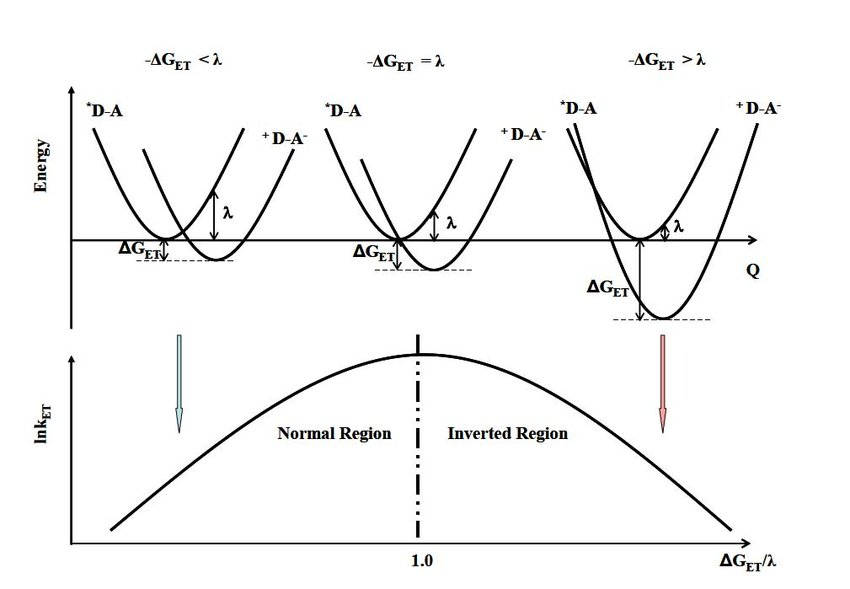
\includegraphics[width=\linewidth]{Marcus}
\end{minipage}
\newpage
\pagestyle{empty}
\addtocounter{page}{-1}	
\section*{\emph{When You See Water}}
\paragraph{By Alice Walker}~
\begin{verse}
	When you see water in a stream\\
	you say: oh, this is stream\\
	water;\\
	When you see water in the river\\
	you say: oh, this is water\\
	of the river;\\
	When you see ocean\\
	water\\
	you say: This is the ocean's\\
	water!\\
	But actually water is always\\
	only itself\\
	and does not belong\\
	to any of these containers\\
	though it creates them.\\
	And so it is with you.
\end{verse}
\end{document}
